% =====================================================================
%  ECONSCHOOL — PROBLEMS SHEET
%  One solved problem (with a TikZ figure) + one near-twin exercise.
%
%  Compile:  pdflatex perfect-complements.tex   (run twice for the footer)
%  No font installation needed: text and maths are Computer Modern
%  (Latin Modern where available), the same maths face the site renders
%  with KaTeX.
% =====================================================================
\documentclass[11pt]{article}

% ---- Fonts ----------------------------------------------------------
% Latin Modern if available (it is on MacTeX); base Computer Modern
% otherwise. Either way the maths face is Computer Modern.
\IfFileExists{lmodern.sty}{\usepackage[T1]{fontenc}\usepackage{lmodern}}{}

% ---- Core packages --------------------------------------------------
\usepackage{amsmath,amssymb}
\usepackage[a4paper,top=2.3cm,bottom=2.4cm,left=2.6cm,right=2.6cm]{geometry}
\usepackage{graphicx}
\usepackage{xcolor}
\usepackage{microtype}
\usepackage{enumitem}

% ---- Figures --------------------------------------------------------
\usepackage{tikz}
\usepackage{pgfplots}
\pgfplotsset{compat=1.18}
\usetikzlibrary{arrows.meta}

% ---- Layout ---------------------------------------------------------
\setlist[enumerate]{leftmargin=1.6em,itemsep=0.35em,topsep=0.3em}
\setlist[itemize]{leftmargin=1.6em,itemsep=0.2em,topsep=0.2em}
\setlength{\parindent}{0pt}
\setlength{\parskip}{0.6em}
\linespread{1.05}

% ---- Brand palette (mirrors src/styles/global.css) ------------------
\definecolor{bg}{HTML}{FAF7F2}             % cream background
\definecolor{ink}{HTML}{2A2620}            % body text
\definecolor{inksoft}{HTML}{4A4239}        % secondary text
\definecolor{inkfaint}{HTML}{7A6F62}       % tertiary / italics
\definecolor{violet}{HTML}{5A1BA6}         % titles
\definecolor{violetsoft}{HTML}{7A4FC4}     % sub-headings
\definecolor{terracotta}{HTML}{A03A2C}     % accents, links, budget line
\definecolor{terracottasoft}{HTML}{C66B5B} % light fills
\definecolor{sage}{HTML}{8AA08A}           % dividers, guide ray
\definecolor{sagesoft}{HTML}{C8D2C0}       % footer rule
\definecolor{rule}{HTML}{E5DDD0}           % hairline rules

% ---- Figure styles --------------------------------------------------
% A small reusable set for the diagrams these sheets need. Add curve
% colours per topic (demand/supply, cost curves, ...) as required.
\pgfplotsset{
  microecon/.style={
    width=8.4cm, height=6.4cm,
    axis lines=middle,
    axis line style={-{Stealth[length=2mm]}, ink},
    tick label style={font=\footnotesize, color=inksoft},
    label style={font=\small, color=inksoft},
    every axis x label/.style={at={(ticklabel* cs:1.02)}, anchor=west},
    every axis y label/.style={at={(ticklabel* cs:1.02)}, anchor=south},
    xmin=0, ymin=0,
    tick align=outside,
    enlargelimits=false,
  },
}
\tikzset{
  indiff/.style={ink, thick},                             % indifference curve
  budget/.style={terracotta, thick},                      % budget line
  optimum/.style={circle, fill=violet, inner sep=1.6pt},  % optimal bundle
}

% ---- Document colour ------------------------------------------------
\color{ink}
\pagecolor{bg}        % cream page; comment out this line for white

% ---- Links ----------------------------------------------------------
\usepackage[hidelinks]{hyperref}
\hypersetup{colorlinks=true, urlcolor=terracotta, linkcolor=terracotta}

% ---- Small reusable pieces ------------------------------------------
\newcommand{\eyebrow}[1]{{\color{terracotta}\textls[110]{\scshape #1}}}
% ES mark: the logo if present, a typographic fallback otherwise.
\newcommand{\esmark}{%
  \IfFileExists{es-logo.png}
    {\raisebox{-0.34\height}{
\includegraphics[height=5mm]{es-logo.png}}}
    {{\color{violet}\fontsize{20}{20}\selectfont\scshape ES}}}
\newcommand{\sagerule}{\par\vspace{0.25em}{\color{sage}\rule{\linewidth}{0.6pt}}\par\vspace{0.15em}}
\newcommand{\heading}[1]{\par\vspace{1.1em}{\color{violet}\large\bfseries #1}\par\vspace{0.25em}}
\newcommand{\subheading}[1]{\par\vspace{0.7em}{\color{violetsoft}\bfseries #1}\par\vspace{0.1em}}
\newcommand{\MU}{\mathrm{MU}}   % upright marginal-utility symbol

% ---- Footer ---------------------------------------------------------
\usepackage{fancyhdr}
\pagestyle{fancy}
\fancyhf{}
\renewcommand{\headrulewidth}{0pt}
\renewcommand{\footrulewidth}{0.4pt}
\renewcommand{\footrule}{{\color{sagesoft}%
  \vskip-\footruleskip\vskip-\footrulewidth
  \hrule height\footrulewidth width\headwidth}}
\fancyfoot[L]{\color{inkfaint}\footnotesize econschool.in}
\fancyfoot[C]{\color{inkfaint}\footnotesize\thepage}
\fancyfoot[R]{\color{inkfaint}\footnotesize youtube.com/@econ.school}

% =====================================================================
\begin{document}

% ---------- Masthead -------------------------------------------------
\noindent
\begin{tabular*}{\linewidth}{@{}l@{\extracolsep{\fill}}r@{}}
  \eyebrow{To go with the lectures} & \esmark
\end{tabular*}
\sagerule

% ---------- Title (replace per sheet) --------------------------------
{\color{violet}\fontsize{26}{30}\selectfont Perfect complements\par}
\vspace{0.2em}
{\color{inkfaint}\itshape Consumer theory \;\textperiodcentered\; Problem~2
 \quad\textperiodcentered\quad
 Video: \href{https://youtu.be/S4v03C39jAI}{youtu.be/S4v03C39jAI}\par}
\sagerule

% =====================================================================
\heading{Solved problem}

A student is making pancakes for the week. Each pancake uses one cup of flour, and a cup of milk is enough for two pancakes; flour with no milk, or milk with no flour, makes no more pancakes. Writing
\begin{itemize}
  \item $x$: cups of flour, at $p_x=4$ each;
  \item $y$: cups of milk, at $p_y=4$ each,
\end{itemize}

the number of pancakes is $u(x,y)=\min\{x,2y\}$. With a budget of \$18 for ingredients, find the optimal bundle $(x^\star,y^\star)$ and illustrate the budget line and the optimal choice in a diagram.

\subheading{Solution}
The student solves
\[
  \begin{aligned}
    \max_{(x,y)\in\mathbb{R}^2_+}\quad & \min\{x,2y\}\\
    \text{s.t.}\quad & 4x+4y\le 18.
  \end{aligned}
\]

Extra flour does nothing without the milk to go with it, and extra milk does nothing without the flour. So at the optimum nothing is wasted,
\[
  x = 2y,
\]
and the budget binds. Substituting $x=2y$ into $4x+4y=18$,
\[
  4(2y)+4y = 12y = 18
  \quad\Longrightarrow\quad
  y=1.5,\qquad x=2y=3.
\]
The optimal bundle is $(x^\star,y^\star)=(3,1.5)$, giving $u=\min\{3,3\}=3$ — three pancakes.

\begin{center}
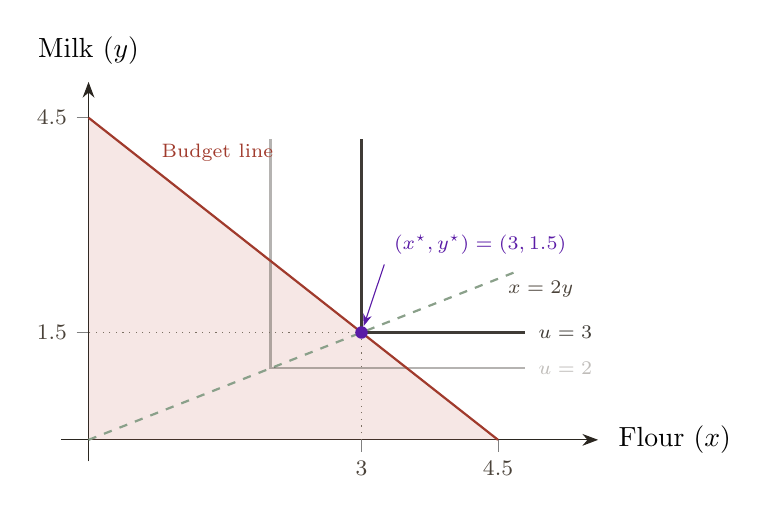
\begin{tikzpicture}
  \begin{axis}[
      microecon,
      xmin=-0.3, xmax=5.6, ymin=-0.3, ymax=5,
      xlabel={Flour ($x$)}, ylabel={Milk ($y$)},
      xtick={3,4.5}, ytick={1.5,4.5},
      clip mode=individual,
  ]
    % Budget set: affordable triangle (0,0)-(4.5,0)-(0,4.5)
    \addplot[draw=none, fill=terracottasoft, fill opacity=0.16]
      coordinates {(0,0) (4.5,0) (0,4.5)} \closedcycle;

    % Ray of no-waste bundles: x = 2y  (the corners line up here)
    \draw[sage, thick, dashed]
      (axis cs:0,0) -- (axis cs:4.7,2.35)
      node[pos=0.97, below right=-2pt, font=\scriptsize, text=inksoft] {$x=2y$};

    % L-shaped indifference curves, corners on x = 2y.
    \draw[indiff, opacity=0.35]                                 % u = 2 (context)
      (axis cs:2,4.2) -- (axis cs:2,1) -- (axis cs:4.8,1)
      node[right=1pt, font=\scriptsize, text=inksoft] {$u=2$};
    \draw[indiff, opacity=0.9]                                  % u = 3 (optimal level)
      (axis cs:3,4.2) -- (axis cs:3,1.5) -- (axis cs:4.8,1.5)
      node[right=1pt, font=\scriptsize, text=ink] {$u=3$};

    % Budget line: 4x + 4y = 18  =>  x + y = 4.5
    \addplot[budget, domain=0:4.5] {4.5 - x}
      node[pos=0.16, above right=-1pt, font=\scriptsize, text=terracotta] {Budget line};

    % Optimum at the kink (3, 1.5): on the budget line and on the ray
    \draw[inkfaint, dotted] (axis cs:3,0) -- (axis cs:3,1.5) -- (axis cs:0,1.5);
    \node[optimum] (opt) at (axis cs:3,1.5) {};
    \node[font=\scriptsize, anchor=south west, text=violet] (optlabel)
      at (axis cs:3.25,2.45) {$(x^\star,y^\star)=(3,1.5)$};
    \draw[-{Stealth[length=1.5mm]}, violet, thin] (optlabel.south west) -- (opt);
  \end{axis}
\end{tikzpicture}
\end{center}
\vspace{-0.2em}
{\color{inkfaint}\footnotesize\itshape
 Figure~1.\enspace With perfect complements the indifference curves are
 L-shaped, their corners lying on the ray $x=2y$ where flour and milk are in
 recipe proportion. The best the budget reaches is the corner of the highest
 L --- on the budget line and on the ray at once --- so nothing is wasted:
 $(x^\star,y^\star)=(3,1.5)$.\par}
\sagerule

% =====================================================================
\heading{Exercise}

A student eats dal and rice in the canteen. One serving of dal with one serving of rice makes a plate; a serving of dal with no rice, or rice with no dal, is no use. Writing
\begin{itemize}
  \item $x$: servings of dal, at $p_x=2$ each;
  \item $y$: servings of rice, at $p_y=1$ each,
\end{itemize}

the number of plates is $u(x,y)=\min\{x,y\}$. The student has \$15 to spend.

\begin{enumerate}
  \item On a diagram, draw the budget set, the budget line, the ray of bundles that waste nothing, and a couple of indifference curves.

  \item Find the utility-maximising bundle $(x^\star,y^\star)$ and the number of plates.
\end{enumerate}

\subheading{Extension: a price rise}

Suppose a poor harvest pushes the price of dal up to $p_x=4$, with the rice price and the \$15 budget unchanged.

\begin{enumerate}
  \setcounter{enumi}{2}
  \item Find the new optimal bundle and the number of plates.
\end{enumerate}

\medskip
{\color{inksoft}\emph{Checking your work.}\enspace To discuss the exercise, join
 the community forum at \href{https://econschool.in}{econschool.in}.\par}

\end{document}
